\documentclass{if-beamer}
% --------------------------------------------------- %
%                  Presentation info	              %
% --------------------------------------------------- %
\title[Pré-distorcedor digital descrito em linguagem VHDL e baseado em polinômio com memória.]{\textbf{Pré-distorcedor digital descrito em linguagem VHDL e baseado em polinômio com memória}}
\subtitle{}
\author[Leonardo de Andrade Santos]{\large \negrito{Leonardo de Andrade Santos}}
\institute[UFPR/PR]{
    \small \textit{Universidade Federal do Paraná} \\
    %\textit{Uned Itaguaí}
}
\date{\the\year}
\logo{

\includegraphics[scale=.1, clip]{ufpr.png}
}
\subject{Presentation subject} % metadata
%trim={<left> <lower> <right> <upper>}
\graphicspath{{figuras/}}
% --------------------------------------------------- %
%                    Title + Schedule                 %
% --------------------------------------------------- %

\begin{document}

\begin{frame}
  \titlepage
\end{frame}

\begin{frame}{Programação}
  \tableofcontents
\end{frame}

\begin{frame}{Introdução}
\begin{itemize}
	\item Devido a evolução dos sistemas de comunicação moveis, que apresentam diversos serviços como aplicações multimídias, desenvolvimento web e aplicações IoT, aumentou a necessidade de desenvolver sistemas cada vez mais energeticamente eficientes;
	\item Largura de banda reservada para sistemas de comunicação sem fio reduzidas;
	\item Modulação na amplitude (AM) sensível a linearidade;
	\item Alternativa para contornar esses obstáculos é a implementação de um DPD em cascata ao Amplificador de Potência (PA);
\end{itemize}
\end{frame}

\begin{frame}{Objetivos}
	Objetivo deste trabalho é desenvolver um circuito integrado dedicado de um DPD.
	\begin{itemize}
		\item Realizar a modelagem de um PA e do DPD com o modelo de polinômio de memória;
		\item Implementar a descrição de hardware em 
		linguagem VHDL;
		\item Fazer o desing do circuito integrado utilizando as ferramentas de design do Cadence;
	\end{itemize}
\end{frame}

% --------------------------------------------------- %
%                      Presentation                   %
% --------------------------------------------------- %

%%%%%%%%%%%%%%%%%%%%%%%%%%%%%%%%%%%%%%%%%%%%%%%%%%%%%%%%%%%%%

\section{Fundamentação teórica}

%%%%%%%%%%%%%%%%%%%%%%%%%%%%%%%%%%%%%%%%%%%%%%%%%%%%%%%%%%%%%

\subsection{Sistema de comunicação}
\begin{frame}{Sistema de comunicação}
	\begin{itemize}
		\item A comunicação sem fio é dividida em 3 sub-sistemas principais:	o transmissor, o meio transmissor (ar), receptor;
		\item O PA é o componente de maior demanda energética por ser o componente que transfere potência da fonte para potência irradiada pela antena
	\end{itemize}
	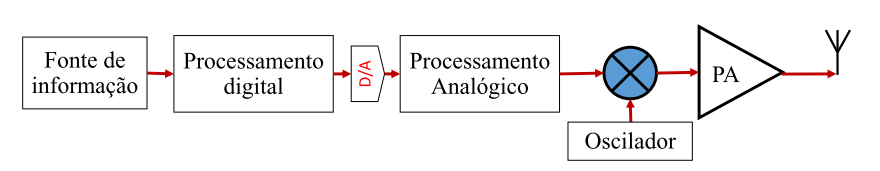
\includegraphics[scale=0.5]{sistematrasmissorpng.png}
\end{frame}

%%%%%%%%%%%%%%%%%%%%%%%%%%%%%%%%%%%%%%%%%%%%%%%%%%%%%%%%%%%%%
\subsection{Problema}
\begin{frame}{Problema}

\begin{minipage}{.49\textwidth}

\begin{itemize}
    \item A curva amarela representa a restrição 
    imposta pela norma regulamentadora;
    \item A curva em verde representa a resposta em frequência do sinal da amplificação;
    antes 
    \item A curva em azul representa o sinal após a amplificação;
    \item As diferenças de densidade de potência nas bandas adjacentes ao canal representam a distorção causada pela não linearidade do PA;
    \item Maior eficiência implica em maior distorção do sinal.
\end{itemize}


\end{minipage}
\begin{minipage}{.49\textwidth}
	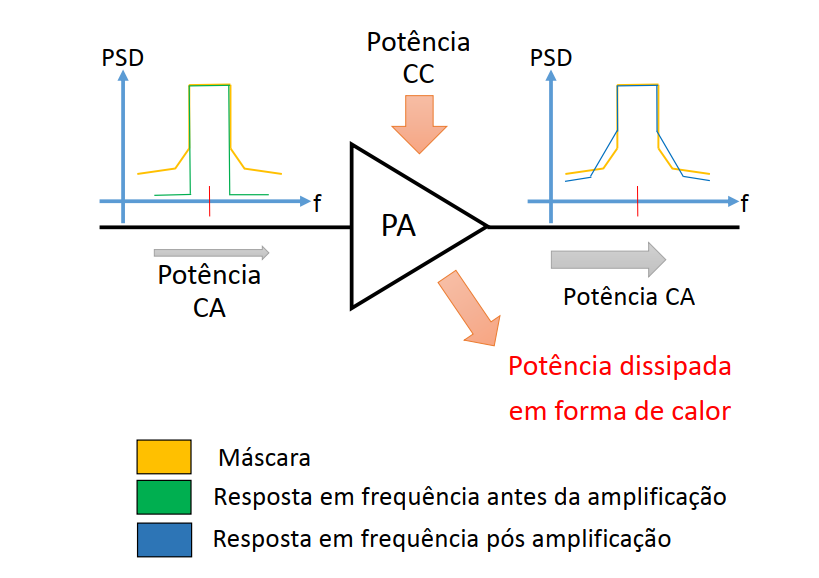
\includegraphics[scale=0.25]{normareg.png}
\end{minipage}

\end{frame}

%%%%%%%%%%%%%%%%%%%%%%%%%%%%%%%%%%%%%%%%%%%%%%%%%%%%%%%%%%%%%
\subsection{Mudar}
\begin{frame}{Mudar}
	
	\begin{minipage}{.49\textwidth}
		
		\begin{itemize}
			\item A característica de transferência não linear do PA 
			é caracterizada pela potência de saída que decai 			1 dB da potência ideal, ou ponto de 1 dB de 
			compressão de ganho (OCP1dB)
			\item  Efeito chamado memória causado devido aos 			componentes armazenadores (capacitâncias de energia e indutâncias), contribuindo significativamente na distorção.
			\item  O DPD, operando em banda base é uma solução 
			eficiente com baixo custo computacional
		
		\end{itemize}
		
		
	\end{minipage}
	\begin{minipage}{.49\textwidth}
		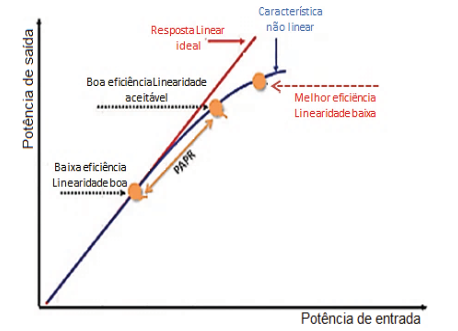
\includegraphics[scale=0.5]{curvasaidaparf.png}
	\end{minipage}
	
\end{frame}


%%%%%%%%%%%%%%%%%%%%%%%%%%%%%%%%%%%%%%%%%%%%%%%%%%%%%%%%%%%%%
\subsection{Pré-distorcedor}
\begin{frame}{Pré-distorcedor}
\begin{minipage}{0.5\textwidth}
		
		\includegraphics[scale=0.5]{DPDCascata.png}
		
	\end{minipage}%
	\hspace{0.04\textwidth}
	\begin{minipage}{0.5\textwidth}
		\begin{itemize}
			\item De maneira sucinta, o DPD é conectado em 
			cascata ao PARF, e é projetado para apresentar a 
			função de transferência inversa ao PARF;
			\item Modelagem física: alto custo computacional;
			\item Modelagem matemática: baixo custo computacional;
			\item Se todos os parâmetros fossem conhecidos, conhecendo o equacionamento completo do circuito, uma função inversa poderia ser encontrada, possivelmente complexa como as séries de Volterra;
		\end{itemize}
	\end{minipage}
\end{frame}
%%%%%%%%%%%%%%%%%%%%%%%%%%%%%%%%%%%%%%%%%%%%%%%%%%%%%%%%%%%%%
\subsection{Séries de Volterra}
\begin{frame}{Séries de Volterra}
		\begin{itemize}
			\item As séries de Volterra são bastante difundidas para a modelagem comportamental;
			\item Não dependerem de parâmetros físicos do circuito; 
			\item Podem ser aplicados na modelagem de qualquer PA;
			\item Apenas medidas das informações de entrada (in) e saída (out) em domínio temporal são necessárias;
		\end{itemize}
		\vspace{0.05\textwidth}
			\[
		y(t) = h_0 + \int h_1(\tau_1) x(t - \tau_1) \, d\tau_1 + \int \int h_2(\tau_1, \tau_2) x(t - \tau_1) x(t - \tau_2) \, d\tau_1 \, d\tau_2 + \cdots
		\]
\end{frame}
%%%%%%%%%%%%%%%%%%%%%%%%%%%%%%%%%%%%%%%%%%%%%%%%%%%%%%%%%%%%%
\subsection{Polinômio de Memória}
\begin{frame}{Polinômio de Memória}
	\begin{minipage}{0.5\textwidth}
		\raggedleft
		\scriptsize
		\begin{equation}
			y(n) = \sum_{p=1}^{P} \sum_{m=0}^{M} h_{p,m} x(n-m) |x(n-m)|^{p-1}
		\end{equation}
			$
				\begin{bmatrix}
					y(1) \\
					y(2) \\
					y(3) \\
					y(4) \\
					y(5)
				\end{bmatrix}
				=
				\begin{bmatrix}
					x(1) & x(0) & x(1)x(1) & x(0)x(0) \\
					x(2) & x(1) & x(2)x(2) & x(1)x(1) \\
					x(3) & x(2) & x(3)x(3) & x(2)x(2) \\
					x(4) & x(3) & x(4)x(4) & x(3)x(3) \\
					x(5) & x(4) & x(5)x(5) & x(4)x(4)
				\end{bmatrix}
				\begin{bmatrix}
					h_{1,0} \\
					h_{1,1} \\
					h_{2,0} \\
					h_{2,1}
				\end{bmatrix}
			$
	
			
		
	\end{minipage}%
	\hspace{0.1\textwidth}
	\begin{minipage}{0.5\textwidth}
		\begin{itemize}
			\item Utilizado na modelagem comportamental simplificada das séries de Volterra.
			\item Considera apenas componentes unidimensionais2;
			\item Modelo compacto;
			\item Baixo custo computacional;
			\item Modelo linear nos coeficientes;
		\end{itemize}
	\end{minipage}
\end{frame}
%%%%%%%%%%%%%%%%%%%%%%%%%%%%%%%%%%%%%%%%%%%%%%%%%%%%%%%%%%%%%
\subsection{Field Port Gate Array (FPGA)}
\begin{frame}{Field Port Gate Array (FPGA)}
	\begin{minipage}{0.5\textwidth}
	
			\includegraphics[scale=0.5]{DPDCascata.png}
		
	\end{minipage}%
	\hspace{0.04\textwidth}
	\begin{minipage}{0.5\textwidth}
		\begin{itemize}
			\item FPGAs compõem uma classe de dispositivos lógicos programáveis;
			\item Eles possuem a capacidade de sintetizar arquiteturas complexas de eletrônica digital;
			\item São descritas como um conjunto de blocos digitais interconectados;
			\item Permite que tarefas possam ocorrer de forma paralela e sequencial;
			
		\end{itemize}
	\end{minipage}
\end{frame}
%%%%%%%%%%%%%%%%%%%%%%%%%%%%%%%%%%%%%%%%%%%%%%%%%%%%%%%%%%%%%
\subsection{Metodologia}
\begin{frame}{Metodologia}
	\begin{minipage}{0.5\textwidth}
		
		%\includegraphics[scale=0.5]{DPDCascata.png}
		
	\end{minipage}%
	\hspace{0.04\textwidth}
	\begin{minipage}{0.5\textwidth}
		 O trabalho foi divido em 4 etapas:
		\begin{itemize}
			\item Etapa 1: Estudos do DPD e modelagem matemática do PA;
			\item Etapa 2: Implementação do DPD em software;
			\item Etapa 3: Implementação do DPD em FPGA;
			\item Etapa 4: Simulação em FPGA;
			\item Etapa 5: Design do Circuito Integrado
			\item Etapa 6: Simulação pós síntese;
		\end{itemize}
	\end{minipage}
	\begin{minipage}{0.5\textwidth}
	
	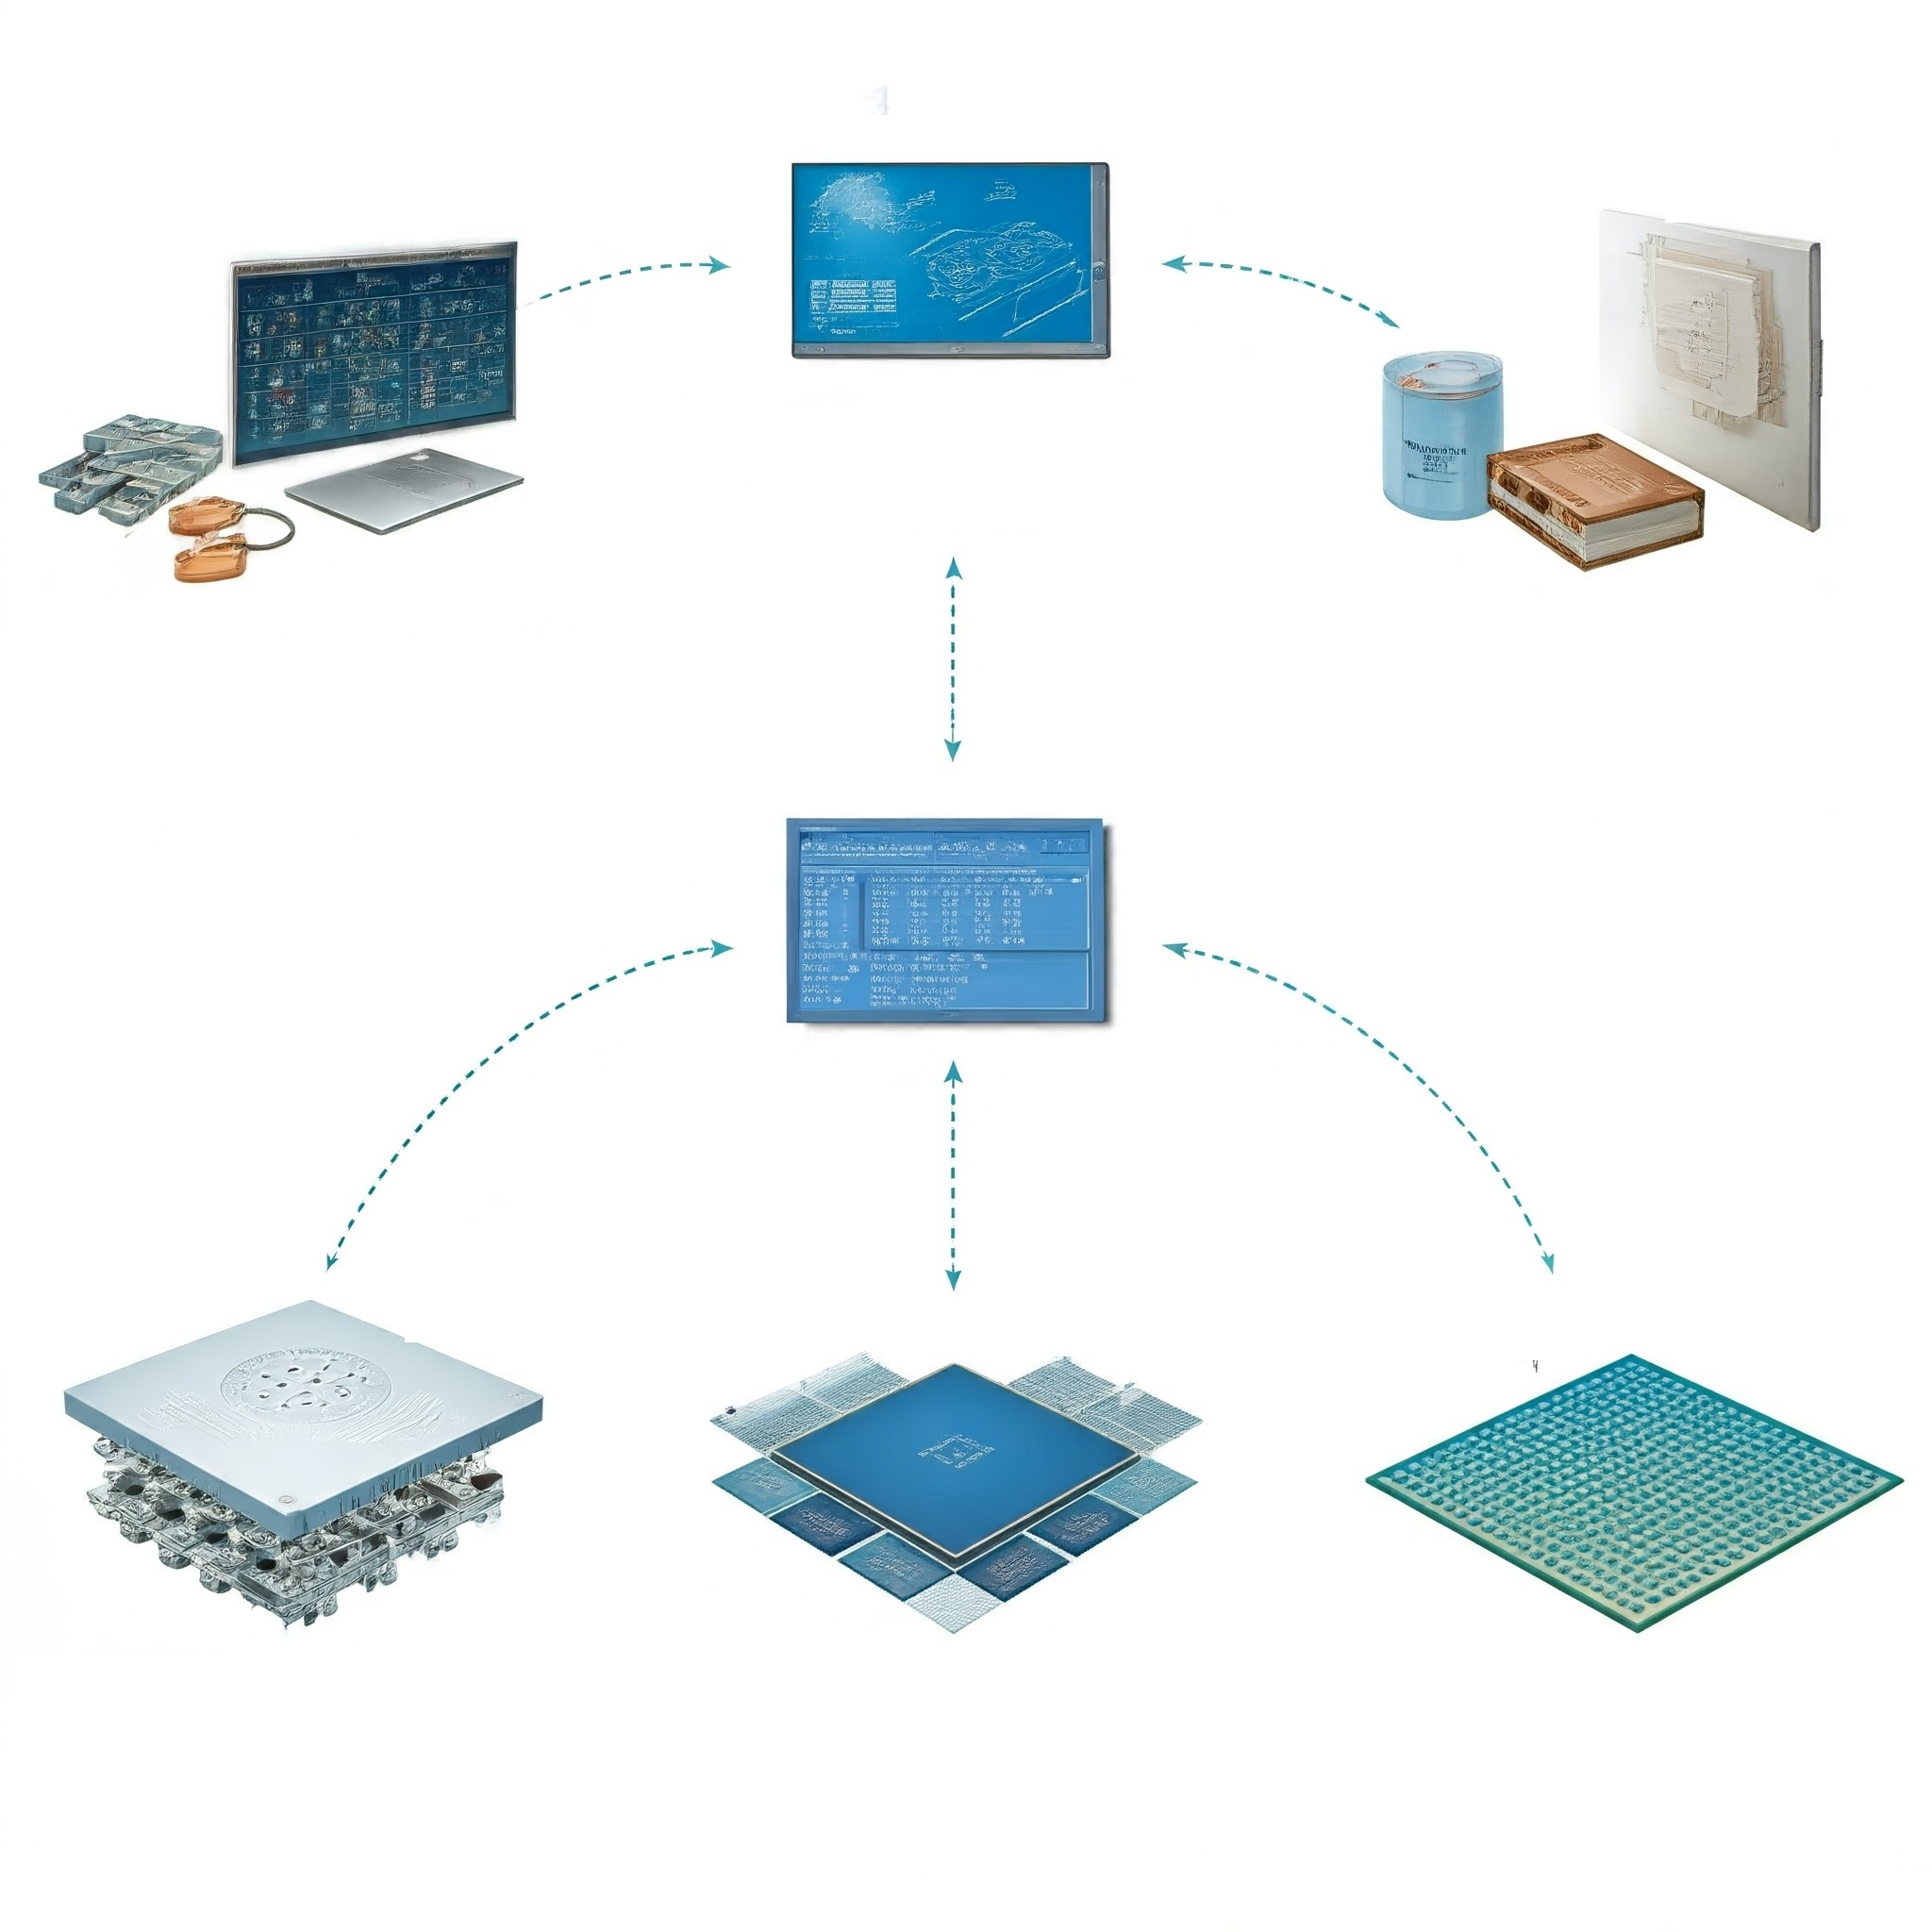
\includegraphics[scale=0.1]{diagrama.png}
	
	\end{minipage}%
\end{frame}
%%%%%%%%%%%%%%%%%%%%%%%%%%%%%%%%%%%%%%%%%%%%%%%%%%%%%%%%%%%%%
\subsection{Dados Utilizados}
\begin{frame}{Dados Utilizados}
	\begin{minipage}{0.5\textwidth}
		
		%\includegraphics[scale=0.5]{DPDCascata.png}
		
	\end{minipage}%
	\hspace{0.04\textwidth}
	\begin{minipage}{0.5\textwidth}
		\begin{itemize}
			\item Amplificador de potência classe AB, HEMT (transistor de efeito de campo de heterojunção) fabricado em tecnologia GaN.
			\item Excitado por um sinal portadora de frequência de 900	MHz;
			\item Modulado por um sinal de envoltória WCDMA 3GPP 3,84 MHz de largura de banda;
			\item Os dados de entrada e saída do amplificador de potência foram medidos usando um analisador de sinal vetorial (VSA) Rohde \& Schwarz FSQ com uma taxa de amostragem de 61,44 MHz;
		\end{itemize}
	\end{minipage}
	\begin{minipage}{0.5\textwidth}
		
		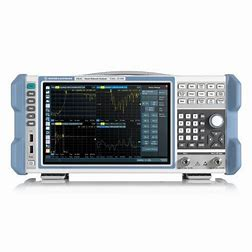
\includegraphics[scale=0.4]{analisador.jpeg}
		
	\end{minipage}%
\end{frame}

\section{Implementação e software}
%%%%%%%%%%%%%%%%%%%%%%%%%%%%%%%%%%%%%%%%%%%%%%%%%%%%%%%%%%%%%
\subsection{Modelagem do PA}
\begin{frame}{Modelagem do PA}
	
	
	\begin{minipage}{0.5\textwidth}
		\begin{itemize}
			\item  Implementação em Python;
			\item Modelagem do PA, com cálculo em vírgula flutuante;
			\item NMSE de -23,57 dB, para um Polinômio de $2^{\circ}$  grau com uma amostra de memória;
		\end{itemize}
	\end{minipage}%
	\hspace{0.04\textwidth}
	\begin{minipage}{0.5\textwidth}
		
		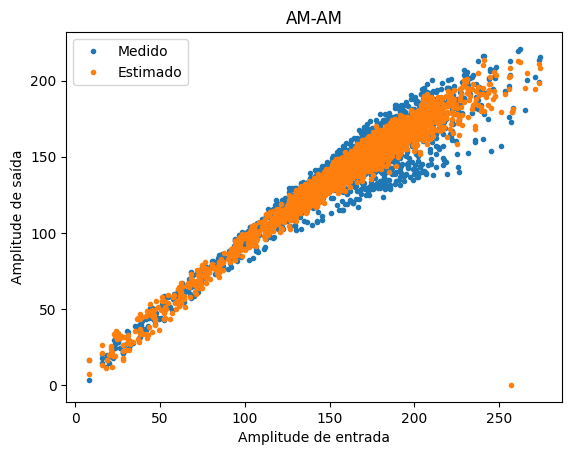
\includegraphics[scale=0.4]{modeloPA.png}
		
	\end{minipage}%
\end{frame}
%%%%%%%%%%%%%%%%%%%%%%%%%%%%%%%%%%%%%%%%%%%%%%%%%%%%%%%%%%%%%
\subsection{Ajuste da Resolução do Sinal}
\begin{frame}{Ajuste da Resolução do Sinal}
	\begin{minipage}{0.5\textwidth}
		\begin{itemize}
			\item Adaptação para realização dos cálculos em vírgula fixa, com uma resolução N de bits;
			\item Inicialmente realizado uma normalização dos dados e em seguida é feitos os cálculos em vírgula fixa Dados DPD com polinômio de memória de grau 2 com um sinal de memória
			\item  Dados DPD com polinômio 	de memória de grau 2 com 
			um sinal de memória
		\end{itemize}
	
		
	\end{minipage}%
	\hspace{0.04\textwidth}
	\begin{minipage}{0.5\textwidth}
	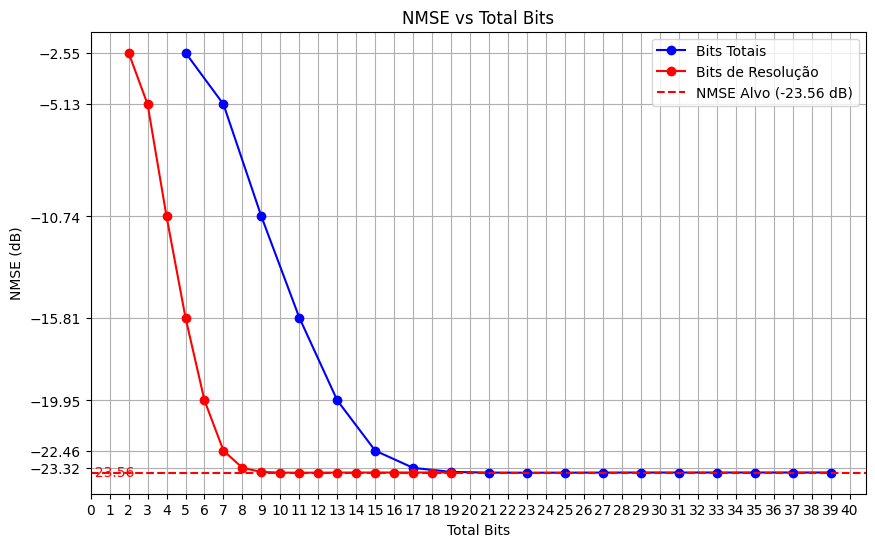
\includegraphics[scale=0.25]{bits.png}
	\end{minipage}
\end{frame}
%%%%%%%%%%%%%%%%%%%%%%%%%%%%%%%%%%%%%%%%%%%%%%%%%%%%%%%%%%%%%
\subsection{Modelagem do DPD}
\begin{frame}{Modelagem do DPD}
	\begin{minipage}{0.5\textwidth}
		\begin{itemize}
			\item Calculo do modulo DPD da mesma forma que do PA, apenas invertendo os dados de entrada com os de saida.
		\end{itemize}
		
		
	\end{minipage}%
	\hspace{0.04\textwidth}
	\begin{minipage}{0.5\textwidth}
		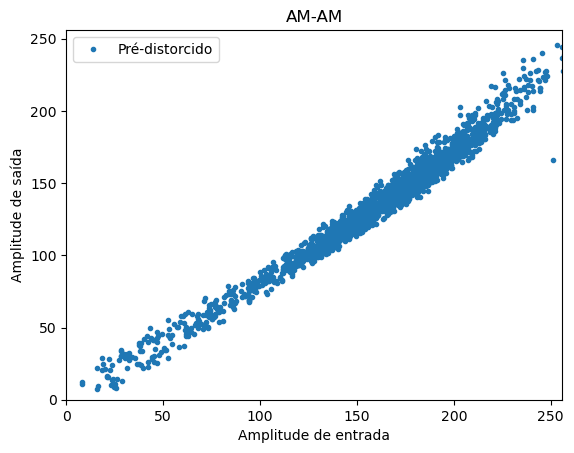
\includegraphics[scale=0.40]{modelodpd.png}
	\end{minipage}
\end{frame}
\section{Implementação em Hardware}
%%%%%%%%%%%%%%%%%%%%%%%%%%%%%%%%%%%%%%%%%%%%%%%%%%%%%%%%%%%%%
\subsection{Desenvolvimento do VHDL}
\begin{frame}{Desenvolvimento do VHDL}
	
		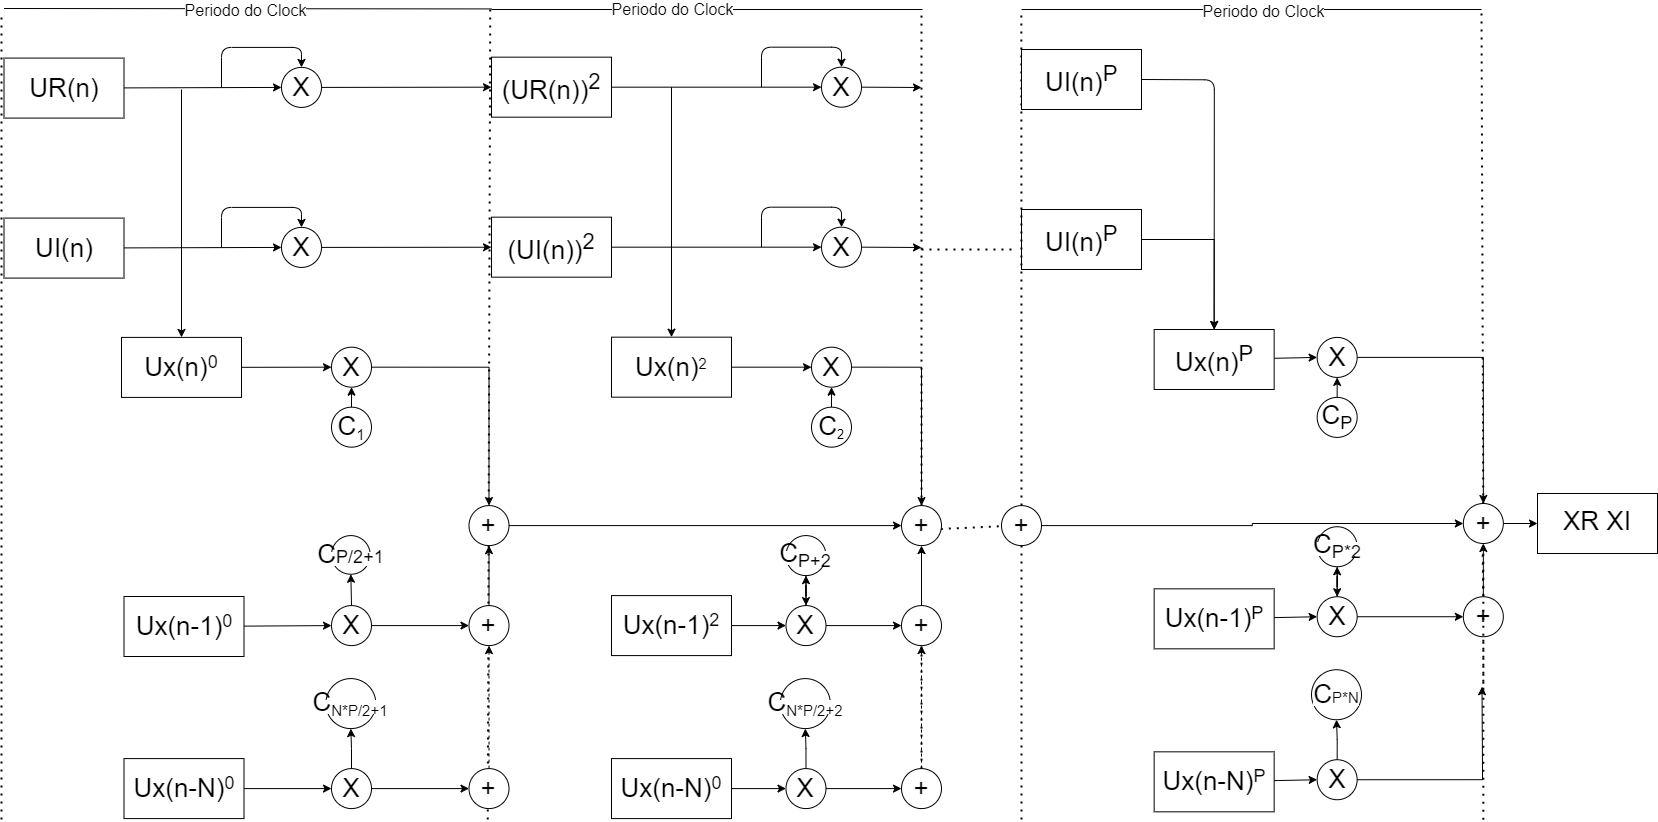
\includegraphics[scale=0.2]{diagrama_process.png}
\end{frame}
%%%%%%%%%%%%%%%%%%%%%%%%%%%%%%%%%%%%%%%%%%%%%%%%%%%%%%%%%%%%%
\subsection{Fluxo de cálculo}
\begin{frame}{Fluxo de cálculo}
	
	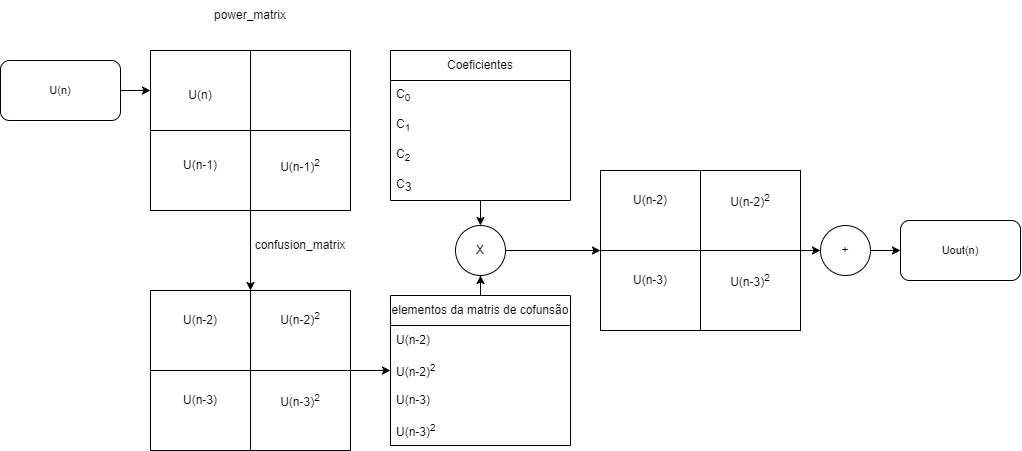
\includegraphics[scale=0.25]{fluxo_de_calculo.png}
\end{frame}
%%%%%%%%%%%%%%%%%%%%%%%%%%%%%%%%%%%%%%%%%%%%%%%%%%%%%%%%%%%%%
\subsection{Resultado simulação FPGA}
\begin{frame}{Resultado simulação FPGA}
	\begin{minipage}{0.5\textwidth}
	\begin{itemize}
		\item FPGA Virtex5 XC5VLX50T;
		\item total de 150 registradores, 692 LUTs e 4 unidades DSP48E;
		\item frequência de operação 61,5 MHz;
	\end{itemize}
	
	
\end{minipage}%
\hspace{0.04\textwidth}
\begin{minipage}{0.5\textwidth}
	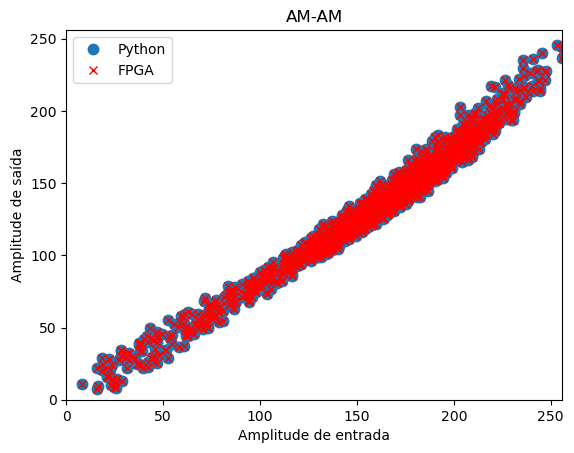
\includegraphics[scale=0.40]{fpgasim.png}
\end{minipage}
\end{frame}
%%%%%%%%%%%%%%%%%%%%%%%%%%%%%%%%%%%%%%%%%%%%%%%%%%%%%%%%%%%%%

\section*{Referências}
\begin{frame}{Referências}
	\setbeamertemplate{navigation symbols}{}
	
		\begin{thebibliography}{}
		\bibitem{John2016} Elton John, ``Modelagem comportamental de amplificadores de potência de radiofrequência usando termos unidimensionais e bidimensionais de séries de Volterra", 2016.
		\bibitem{Kenington2000} Peter Kenington, ``High Linearity RF Amplifier Design", 2000.
		\bibitem{Cripps2006} Steve Cripps, ``RF Power Amplifiers for Wireless Communications", 2006.
		\bibitem{Chavez2018} Joel Huanca Chavez, ``Estudo comparativo entre as arquiteturas de identificação de pré-distorcedores digitais através das aprendizagens direta e indireta", 2018.
		\bibitem{Pedroni2010} Volnei Pedroni, ``Eletrônica Digital e VHDL ", 2010.
		\bibitem{Gonçalves2009} Eduardo Gonçalves de Lima and Giovanni Ghione, ``Behavioral modeling and digital base-band predistortion of RF power amplifiers", 2009.
		\bibitem{Schuartz2017} Luis Schuartz and Eduardo Lima, ``Polinômios com Memória de Complexidade Reduzida e sua Aplicação na Pré-distorção Digital de Amplificadores de Potência", 2017.
		
		\bibitem{Bonfim2016} Elton J Bonfim and Eduardo G De Lima, ``A Modified Two Dimensional Volterra-Based Series for the Low-Pass Equivalent Behavioral Modeling of RF Power Amplifiers", vol. 47, pp. 27-35, 2016.
		
		%	\bibitem{Wayne} Wayne Wolf, ``Modern VLSI Design: IP-Based Design, Fourth Edition", Prentice Hall Modern Semiconductor Design Series.
		%	\bibitem{Raychaudhuri2012} Dipankar Raychaudhuri and Narayan B. Mandayam, ``Frontiers of Wireless and Mobile Communications", Proceedings of the IEEE, vol. 100, no. 4, pp. 824-840, 2012.
		%	\bibitem{Silva2013} Pedro Silva, ``Combinação entre pré-distorção digital e redução de fator de crista para linearização de amplificadores de potência para sistemas de telecomunicações móveis", 2013.
		%	\bibitem{Lima2009} Eduardo Gonçalves de Lima and Giovanni Ghione, ``Behavioral modeling and digital base-band predistortion of RF power amplifiers", 2009.
		%	\bibitem{CMOS2010} Neil H.E.Weste and David Money Harris, ``CMOS VLSI Design: A Circuits and Systems Perspective (4th Edition)", 2010.
		
		%	\bibitem{Pedroni2020} Volnei Pedroni, ``Circuit design with VHDL", 2020.
	\end{thebibliography}

\end{frame}
%%%%%%%%%%%%%%%%%%%%%%%%%%%%%%%%%%%%%%%%%%%%%%%%%%%%%%%%%%%%%


%%%%%%%%%%%%%%%%%%%%%%%%%%%%%%%%%%%%%%%%%%%%%%%%%%%%%%%%%%%%%

\end{document}
